\label{chap:discussion}

\section{Lengths of Tracks}
 %%%%%%%%%%%%%%%%%%%%%%%%%%%%%%%%%%%%%%%%%%%%%%%%%%%%%%%%%%%%%%%%%%%%%%%%%%%%%%%%%
\begin{marginfigure}
	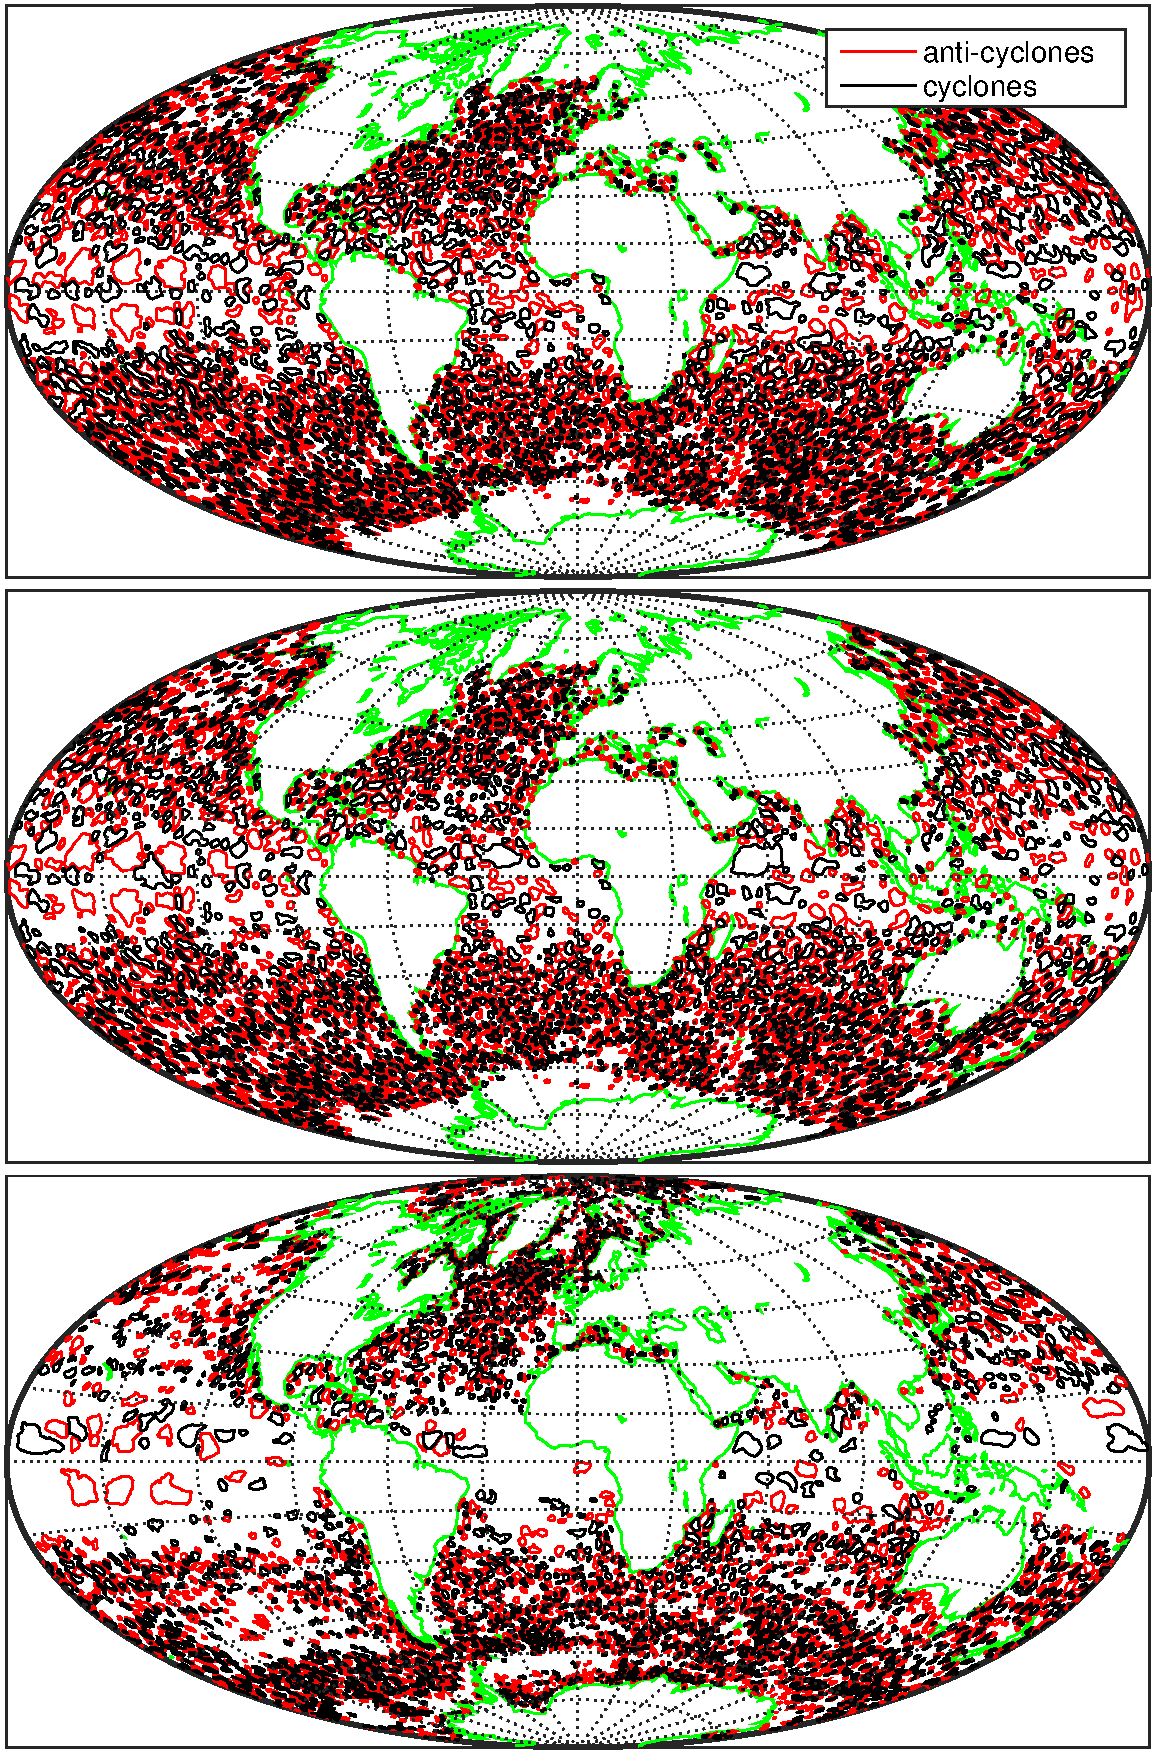
\includegraphics[]{allEddies-aviIaviIIpop7II}
	\caption{All contours that passed the filtering procedure for one exemplary time-step. Top: \aviI. Mid: \aviII. Bottom: \popSevenII.}
	\label{fig:allEddies-aviIaviIIpop7II}
\end{marginfigure}
 %%%%%%%%%%%%%%%%%%%%%%%%%%%%%%%%%%%%%%%%%%%%%%%%%%%%%%%%%%%%%%%%%%%%%%%%%%%%%%%%%
\newthought{The most apparent difference } between the results of the \href{box:MI}{two detection-methods } is the abundance of long-lived eddies resulting from the \MI-method.
This discrepancy must logically be caused by the two different contour-shape-testing procedures (\cref{box:MII,filter:shape}), since it is here where the main difference between the two methods' algorithms lies.

\newthought{The } \MI-method is the more lenient one, as all it checks for, is whether the contour is of sufficiently compact form. The only shapes that are dismissed are long, thin elongated structures. This means that \eg an eddy track can more easily \footnote{as long as the similarity-criterion is not violated.} survive situations in which two eddies merge into one or those in which one is split into two or situations in which mean current gradients distort the vortex.\\ There could also be the situation in which an old, weak eddy fades, yet another one emerges in sufficient proximity. These two events would not even have to coincide at the exact same time, as long as some short-lived coherent structure, of which there is an abundance \footnote{see \cref{fig:allEddies-aviI}} at any given time-step throughout the world ocean, acted as a \textit{bridge} to fill the gap.

\newthought{The } \MII-method is conceptually different in that it is based on the assumption that a distinct coherent vortex need \textit{per definition} to be more or less circular. It will therefor be more likely to regard \eg the situation in which one eddy merges with another as a situation of 3 eddies in total; \textbf{two} that have just died to create \textbf{one} new one.
The focus here is more on the propagation of distinct circular geostrophic vortices whereas the focus in the \MI-method is more general on coherent local depressions respective elevations in SSH. Unfortunately the time-frame of this work did not allow to test to which degree tracers \footnote{in the model data.} found within tracked eddies remained within the eddy over time. This could further clarify the assumption that the \MI-method may be better at tracking water-mass advecting entities, with less jumps between bodies of water within one track.

\section{Scales}
% %%%%%%%%%%%%%%%%%%%%%%%%%%%%%%%%%%%%%%%%%%%%%%%%%%%%%%%%%%%%%%%%%%%%%%%%%%%%%%%%%
\begin{marginfigure}
	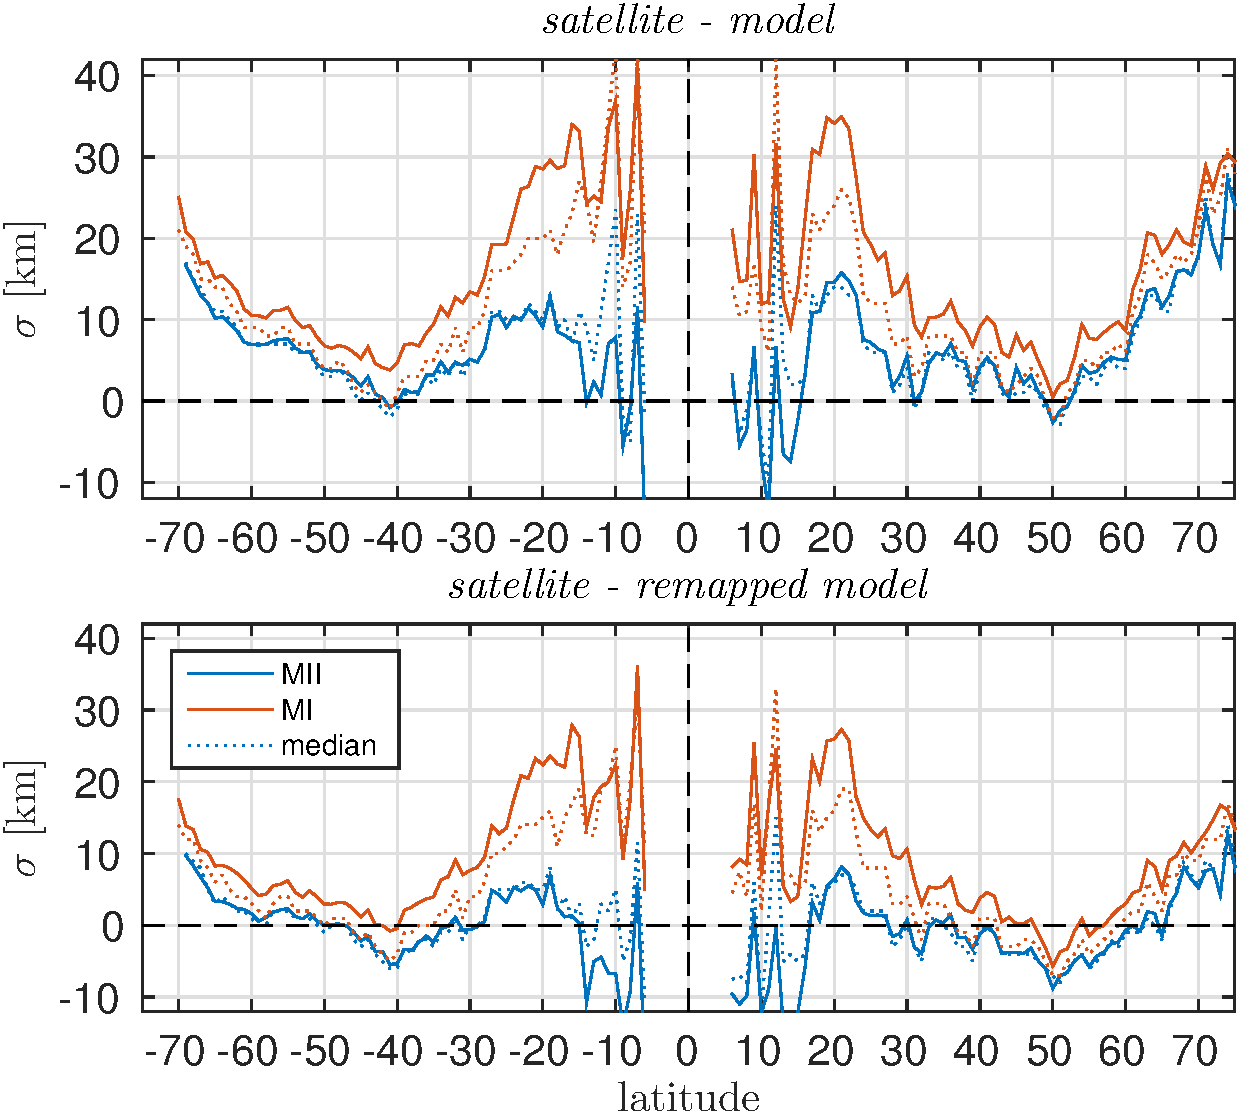
\includegraphics[]{sigmaSatDiffsINTRSCT}
	\caption{Differences in zonal mean \scale between \AVI/\POP and \AVI/downsampled \POP. Means/Medians are built zonally over only those $\deg{1}\times\deg{1}$-bins that feature data in both sets \ie the intersection of $lat+1\i \; lon$ of both sets. }
	\label{fig:sigmaSatDiffsINTRSCT}
\end{marginfigure}
% %%%%%%%%%%%%%%%%%%%%%%%%%%%%%%%%%%%%%%%%%%%%%%%%%%%%%%%%%%%%%%%%%%%%%%%%%%%%%%%%%

\newthought{Interestingly }, even in the \aviI results, the horizontal eddy scale \scale differs from that presented by \citet{Chelton2011}. For latitudes $\gtrsim\abs{\deg{25}}$ the zonal mean here is smaller than theirs while for low latitudes it is higher (see \cref{fig:ScheltsAll}). The reason for this discrepancy is suspected to stem from the special method by which \scale is determined by our algorithm.
As outlined in \cref{filter:dynscale}, here \scale is half the mean of zonal and meridional distances between the first two local extrema of the first derivative of interpolated 4th-order fourier fits to the SSH data around the eddy's \CoV .
The motivation to use fits instead of the SSH directly was on the one hand to avoid noise complicating correct determinations of the 2nd differential zero-crossings and on the other hand to tackle the problem of coarse resolution, especially so for high latitudes where \scale seems to become as small as only twice the distance between data points. At this resolution the \textit{Gaussian RMS width} of an eddy would amount to only 5 data points. Since \scale is generally smaller in the higher-resolution \\POP-data anlyses, we hypothesize that the scales by \citeauthor{Chelton2011} are biased high for high latitudes. Question remains to what degree this bias is inherent to the \AVI product \ie as a smearing effect from the interpolation of multiple coarse satellite data. Or whether it is attributable entirely to the particular method by which the diameter/area of the zero-vorticity contour is estimated.

% %%%%%%%%%%%%%%%%%%%%%%%%%%%%%%%%%%%%%%%%%%%%%%%%%%%%%%%%%%%%%%%%%%%%%%%%%%%%%%%%%
\begin{marginfigure}
	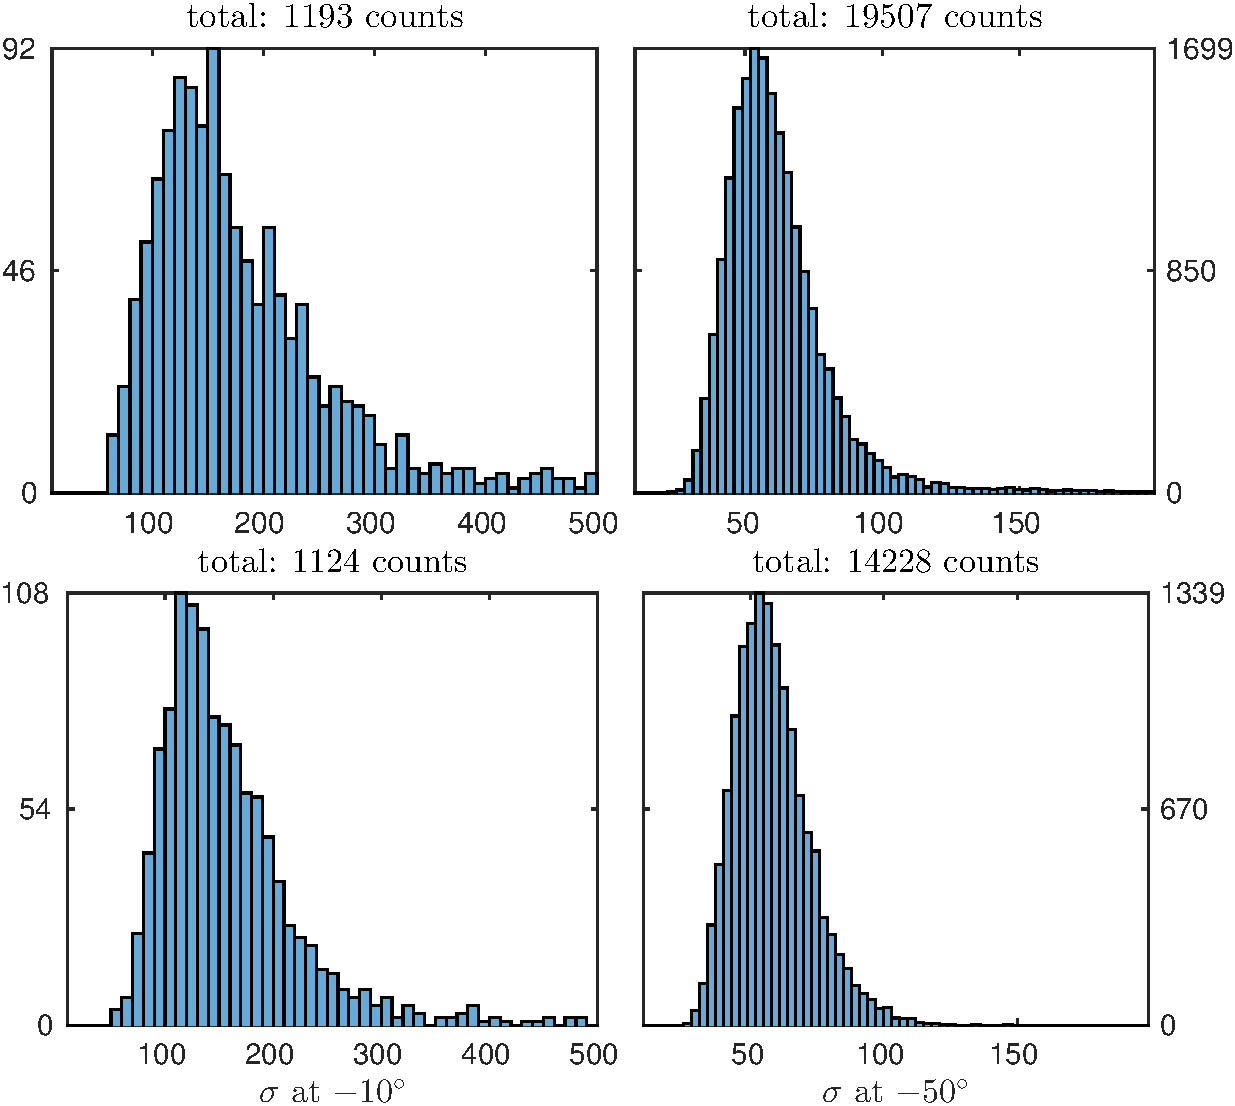
\includegraphics[]{hist-sigmaAt-both-aviIaviII}
	\caption{Eddy count at one point in time for one fully zonal $\deg{1}$-bin. Top: \aviI. Bottom: \aviII. The tropical spectrum is broad yet with strong positive skewness \ie oriented towards smaller scales. In high latitudes the standard deviation is smaller. The \MI method yields more large eddies.}
	\label{fig:hist-sigmaAt-both-aviIaviII}
\end{marginfigure}
% %%%%%%%%%%%%%%%%%%%%%%%%%%%%%%%%%%%%%%%%%%%%%%%%%%%%%%%%%%%%%%%%%%%%%%%%%%%%%%%%%

\newthought{With regard } to the lower latitudes two important aspects need to be considered:
\begin{enumerate}
	\item
	The analyes yield generally low eddy activity in the tropics. Hence the results are less robust in this region \textit{a priori}.
	\item
	The standard deviation in \scale is particulary broad in the tropics (see \cref{fig:hist-sigmaAt-both-aviIaviII}). As a matter of fact it appears as though there might be two different types of eddies. One type analoguous to all high-latiude eddies and a new one of much larger scale. Because these larger eddies have generally low $\IQ$-values they are filtered from the \MII analyses, resulting in smaller tropical \scale. Their more chaotic shape might, due to the different methods to determine \scale, also have to do with why mean tropical \scale is larger here than in \citet{Chelton2011}.
\end{enumerate}
% %%%%%%%%%%%%%%%%%%%%%%%%%%%%%%%%%%%%%%%%%%%%%%%%%%%%%%%%%%%%%%%%%%%%%%%%%%%%%%%%%
%\begin{marginfigure}
	%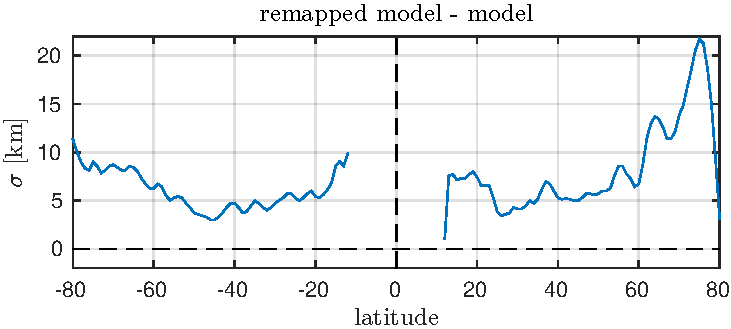
\includegraphics[]{sigmaP2aMinusMod}
	%\caption{\TODO{caption}}
	%\label{fig:TODO}
%\end{marginfigure}
% %%%%%%%%%%%%%%%%%%%%%%%%%%%%%%%%%%%%%%%%%%%%%%%%%%%%%%%%%%%%%%%%%%%%%%%%%%%%%%%%%

% %%%%%%%%%%%%%%%%%%%%%%%%%%%%%%%%%%%%%%%%%%%%%%%%%%%%%%%%%%%%%%%%%%%%%%%%%%%%%%%%%
\begin{wrapfigure}{r}{.6\textwidth}
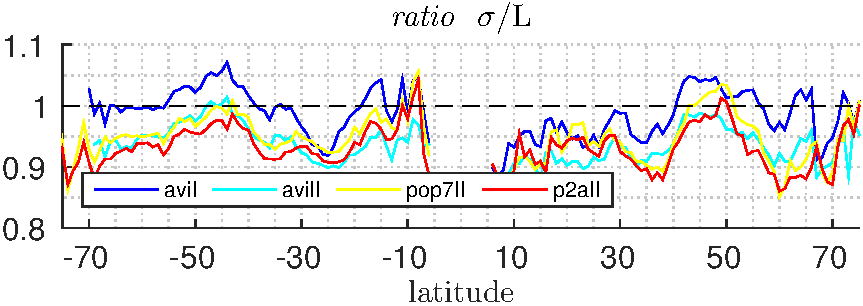
\includegraphics[width=0.6\textwidth]{S-scaleRatios-aviI}
\caption{ Ratios if \scale to \L  (see \cref{filter:chstuff})}
\label{fig:S-scaleRatios-aviI}
\end{wrapfigure}
% %%%%%%%%%%%%%%%%%%%%%%%%%%%%%%%%%%%%%%%%%%%%%%%%%%%%%%%%%%%%%%%%%%%%%%%%%%%%%%%%%

\newthought{The } \popSevenII analysis yields somewhat simlilar \scale for low latiudes \footnote{Note that due to the lack of tropical eddies the estimates of \scale are rather uncertain for the \POP analyses.}, yet significantly smaller values for high latitudes. The question therefor is whether this discrepancy is a result of the lower resolution of the satellite data \ie that eddies are too small to be resolved by the \AVI product in high latitudes or whether it is attributable to the model data as in a systematic bias du to incomplete/poorly parameterised model physics. This question was the primary motivation for the \pToaII-analysis. The idea here was to down-size the \POP data to the geometry of the \AVI grid in order to test whether this would raise \scale to that from the satellite results. \Cref{fig:sigmaSatDiffsINTRSCT} shows that the down-sampling did indeed decrease the discrepancy in \scale to respective \AVI analysis, as long as those regions that are unique to either data set are excluded. Between $\pm \deg{25}$ and $\pm \deg{65}$ the difference is no larger than $\pm \km{5}$. This came as a surprise because since \scale stems from fourier fits of SSH, we expected the original frequencies to be, at least to some extent, conserved in the down-sampled data.

% %%%%%%%%%%%%%%%%%%%%%%%%%%%%%%%%%%%%%%%%%%%%%%%%%%%%%%%%%%%%%%%%%%%%%%%%%%%%%%%%%
\begin{marginfigure}
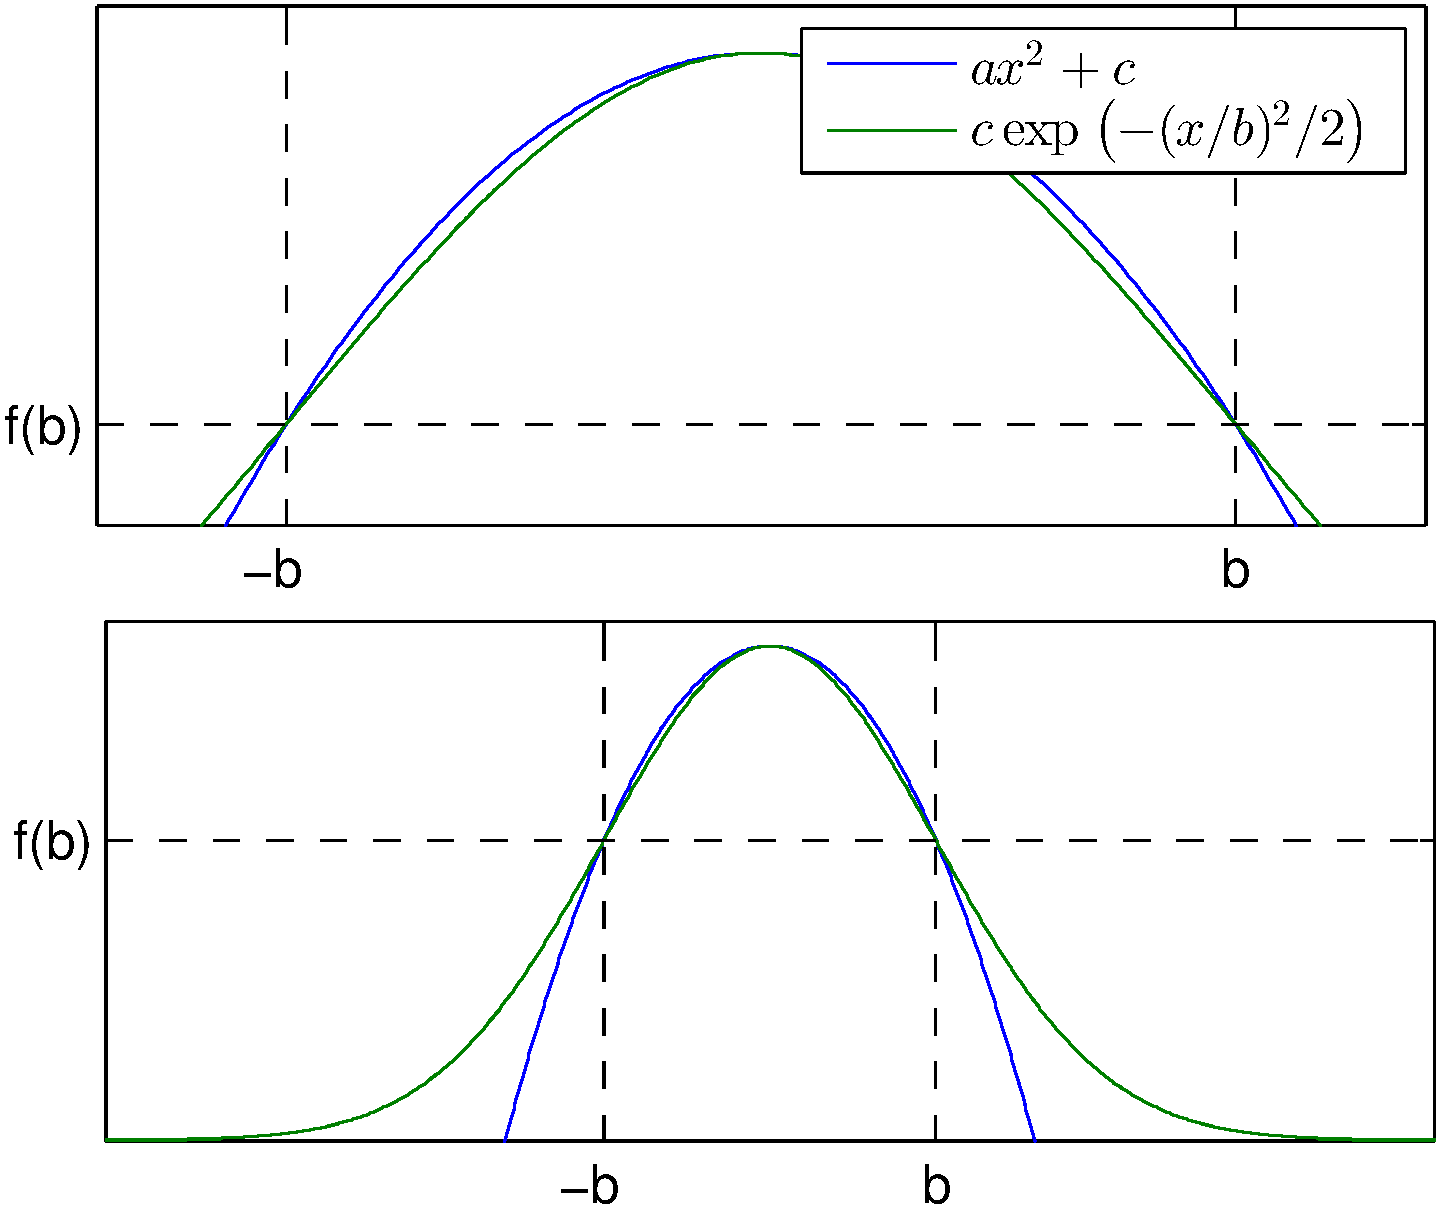
\includegraphics[]{gaussVSquadSmaller}
\caption{The upper part of a Gaussian profile can appear similar to a quadratic one.}
\label{fig:gaussVSquad}
\end{marginfigure}
% %%%%%%%%%%%%%%%%%%%%%%%%%%%%%%%%%%%%%%%%%%%%%%%%%%%%%%%%%%%%%%%%%%%%%%%%%%%%%%%%%


\newthought{The } \MI detection method a priori assumes that an eddy is more or less detected at its asymptotic \textit{floor} \ie in the case of an \AC at the \textit{foot of the mountain}.
 The idea of the $\IQ$-based method on the other hand is to assume that the situation of a single well-defined eddy sitting on an otherwise smooth, flat sea surface, which would be necessary for the contour algorithm to find a closed contour describing the outermost perimeter of said single vortex, is unrealistic. Instead the approach is to look for distinct, sufficiently circular \textit{caps} of SSH-hills/valleys that consistently \textit{wade} through all other weaker geostrophic noise surrounding it. \TODO{ why gaussian or quad?}


% %%%%%%%%%%%%%%%%%%%%%%%%%%%%%%%%%%%%%%%%%%%%%%%%%%%%%%%%%%%%%%%%%%%%%%%%%%%%%%%%%
\section{Drift Speeds}

\newthought{Zonal mean drift speeds } of all \AVI results agree well with those presented by \citet{Chelton2011} (see \cref{fig:ScheltsAll}), suggesting that the tracking procedures are relatively robust for both the \MI and \MII methods.

\newthought{The } \popSevenII results yield generally smaller magnitudes of $u$.
The apparent drop in magnitude at $\sim\deg{12}$N is most likely due to erronuous inter-time-step eddy-associations. In that region, the combination of extreme sparsity of results, large time-step, large \scale, low amplitude and high (theoretical) drift speed make robust determinations of$u$ practically impossible.
Yet the tendency for lower magnitudes in $u$, albeit less stark, is also true for higher latitudes.
The meridional drift speeds are calculated via gradients of \textit{polyfits} to the \CoV-locations on the surface of a spherical earth. This method was tested thoroughly and its robustness is further validated by the fact that the weaker $u$ remains approximtely the same after downsampling for the \pToaII run.

\newthought{From } \cref{eq:cush1} we know that at first approximation (planetary lift)
\begin{align}
u
&\sim
\beta \left( 	\frac{NH}{f_{0}}  \right)^{2}
\end{align}
Since $\beta, H$ and $f$ should be set realisticaly in \POP, it appears that the, evidently unrealsitic, drift speeds in the model results stem from an unrealisitc or poorly resolved (only 42 vertical layers in \POP) density stratification $\dpr{\rho}{z}$.

\begin{marginfigure}
	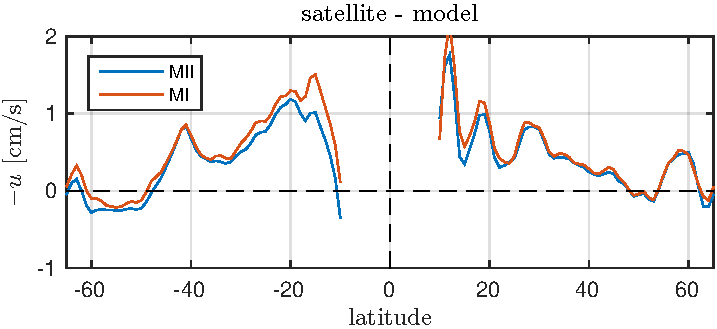
\includegraphics[]{velSatMinusMod}
	\caption{\scriptsize{\aviI/\aviII minus \popSevenII of zonal drift speed means.}}
	\label{fig:velSatMinusMod}
\end{marginfigure}
% %%%%%%%%%%%%%%%%%%%%%%%%%%%%%%%%%%%%%%%%%%%%%%%%%%%%%%%%%%%%%%%%%%%%%%%%%%%%%%%%%
% %%%%%%%%%%%%%%%%%%%%%%%%%%%%%%%%%%%%%%%%%%%%%%%%%%%%%%%%%%%%%%%%%%%%%%%%%%%%%%%%%
\begin{marginfigure}
		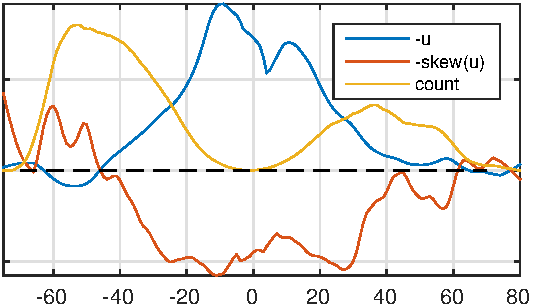
\includegraphics[]{Skew-aviI}
		\caption{\scriptsize{Skewness (red) of $-u$ for \aviI. The spectrum leans towards high westward values in low latitudes. In the ACC the distribution reverses indicating the existence of sporadic events of strong eastward advection by the mean flow. (Note: Everything normalised to fit all in one frame.)}}
		\label{fig:SkewAviI}
\end{marginfigure}
% %%%%%%%%%%%%%%%%%%%%%%%%%%%%%%%%%%%%%%%%%%%%%%%%%%%%%%%%%%%%%%%%%%%%%%%%%%%%%%%%%
